%\documentclass[tikz, border=5pt]{standalone}
\begin{document}
	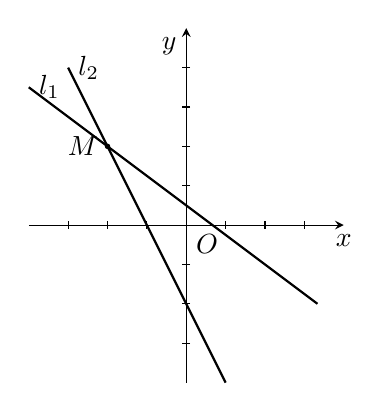
\begin{tikzpicture}[>=stealth, scale=0.5]
		% 1. 绘制坐标轴
		\draw[->] (-4,0) -- (4,0) node[below] {$x$}; % x轴(带箭头和标签)
		\draw[->] (0,-4) -- (0,5) node[below left] {$y$}; % y轴(带箭头和标签)
		\node at (0,0) [below right] {$O$};          % 原点标记
		
		% 绘制所有小刻度线(从 -1 到 2,每隔 1 单位画竖线)
		\foreach \x in {-3,-2,...,3} {
			\draw (\x, 0.1) -- (\x, -0.1) ;  % 小竖线(长 0.2 单位)
		}
	\foreach \y in {-3,-2,...,4} {
		\draw (0.1,\y) -- (-0.1,\y) ;  % 小竖线(长 0.2 单位)
	}
	
	% 2. 绘制直线  l1 虚线 4y=-3x+2 
	\draw[thick] (10/3,-2) -- (-4, 3.5) node[ right] {$l_1$}; % 虚线部分
	% 2. 绘制直线  l 2虚线 y=-2x-2 
	\draw[thick] (1,-4) -- (-3, 4) node[ right] {$l_2$}; % 虚线部分
	
	% 3. 标记各点(M)
	\fill (-2,2) circle (2pt) node [left] {$M$};
	
	\end{tikzpicture}
\end{document}
